\documentclass[12pt,a4paper]{article}
\usepackage[utf8x]{inputenc}
\usepackage[english,hebrew]{babel}
\usepackage{graphicx}
\usepackage{verbatim}
\usepackage{url}

\graphicspath{{images/}}


\textwidth=15.5cm
\textheight=23cm
\topmargin=0pt
\headheight=0pt
\oddsidemargin=2em
\headsep=0pt
\parindent=0pt
\renewcommand{\baselinestretch}{1.1}
\setlength{\parskip}{0.3\baselineskip plus 1pt minus 1pt}

\begin{document}
\thispagestyle{empty}

\selectlanguage{hebrew}

\begin{center}
\textbf{\Huge סדרות}

\bigskip
\bigskip

\textbf{\Large מוטי בן-ארי}

\bigskip

\textbf{\Large המחלקה להוראת המדעים}

\bigskip

\textbf{\Large מכון ויצמן למדע}

\bigskip

\url{http://www.weizmann.ac.il/sci-tea/benari/}

\bigskip

\end{center}

\selectlanguage{english}

\begin{center}
\sffamily\copyright{}\  2018 by Moti Ben-Ari.
\end{center}

\begin{footnotesize}
\sffamily
This work is licensed under the Creative Commons Attribution-ShareAlike 3.0 Unported License. To view a copy of this license, visit \url{http://creativecommons.org/licenses/by-sa/3.0/} or send a letter to Creative Commons, 444 Castro Street, Suite 900, Mountain View, California, 94041, USA.
\end{footnotesize}

\bigskip

\begin{center}

\includegraphics[width=.2\textwidth]{../../by-sa.png}
\end{center}

\bigskip
\bigskip
\bigskip

\selectlanguage{hebrew}

אני מודה לרונית בן-בסט לוי על הערותיה המועילות.
\newpage


במסמך זה ננתח את השאלות על סדרות בבחינות הבגרות, שאלון
$806$.
נחפש תבניות המופיעות בשאלות ונצביע על דרכים לפתרונן. בסוף המסמך רשמתי המלצות למתמודד עם סדרות.


%%%%%%%%%%%%%%%%%%%%%%%%%%%%%%%%%%%%%%%%%%%%%%%%%%%%%%%%%%%%%%%%%%%


\textbf{\R{
חורף תשע"ד
}}
\begin{center}
\selectlanguage{english}
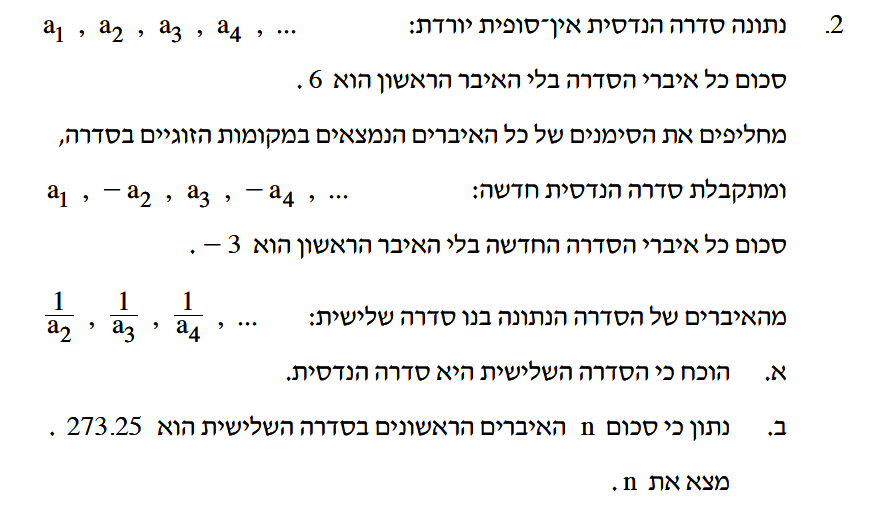
\includegraphics[width=.9\textwidth]{winter-2014-2}
\end{center}
\vspace{-2ex}
סעיף א. המנה של הסדרה השלישית קבועה כי נתון שהסדרה הראשונה הנדסית:
\[
\frac{1/a_{n+1}}{1/a_n}=\frac{a_n}{a_{n+1}}
\]
סעיף ב. נתון:
\[
\frac{a_2}{1-q}=6,\quad\quad \frac{-a_2}{1-(-q)}= -3,\quad\quad \frac{1}{a_2}\cdot\frac{\displaystyle\frac{1}{q^n}-1}{\displaystyle\frac{1}{q}-1}=273.25\,.
\]
משתי הנוסחות הראשונות נחשב
$q=\frac{1}{3}$
ו-%
$a_2=6\cdot \left(1-\frac{1}{3}\right)=4$.
נציב בנוסחה השלישית ונקבל
$3^n=2187$.
בדיקת חזקות של
$3$
מראה ש-%
$n=7$.

%%%%%%%%%%%%%%%%%%%%%%%%%%%%%%%%%%%%%%%%%%%%%%%%%%%%%%%%%%%%%%%%%%%
\bigskip

\textbf{\R{
קיץ תשע"ד, מועד א
}}

\begin{center}
\selectlanguage{english}
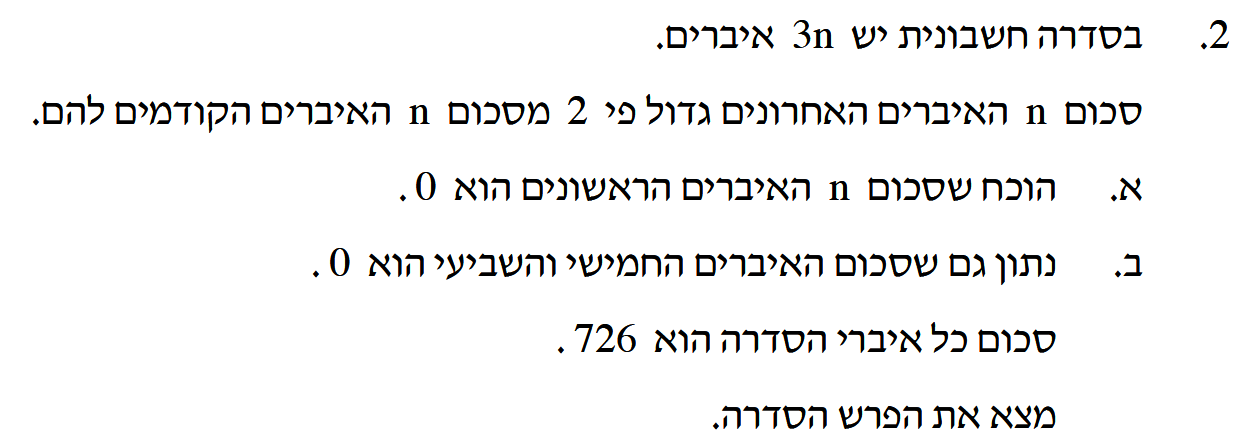
\includegraphics[width=.9\textwidth]{summer-2014a-2}
\end{center}

כדי לדייק עם האינדקסים כדאי לרשום את הסדרה עם סימון של הסדרות החלקיות:
\[
\underbrace{
\overbrace{\rule{0pt}{8pt}a_1, a_2, \ldots, a_n}^{S_1},
\overbrace{\rule{0pt}{8pt}a_{n+1}, a_{n+2}, \ldots, a_{2n}}^{S_2},
\overbrace{\rule{0pt}{8pt}a_{2n+1}, a_{2n+2}, \ldots, a_{3n}}^{S_3}
}_{S_{3n}}\,.
\]
סעיף א. נסכם כל תת-סדרה בנפרד כאשר ההפרשים שווים אבל האיברים הראשונים שונים:
\[
a_1,\quad\quad a_{n+1} = a_1 + nd, \quad\quad a_{2n+1} = a_1 + 2nd\,.
\]
לפי היחס הנתון בין הסכומים:
\[
\renewcommand{\arraystretch}{1.2}
\begin{array}{lll}
S_3&=&2S_2\\
\frac{n}{2}(2(a_1+2nd)+(n-1)d)&=&2\cdot \frac{n}{2}(2(a_1+nd)+(n-1)d)\\
2a_1+(5n-1)d&=&4a_1+(6n-2)d\\
2a_1+(6n-5n-2+1)d&=&0\\
2a_1+(n-1)d&=&0\,.
\end{array}
\]
הביטוי בצד השמאלי של המשוואה האחרונה הוא הסכום 
$S_1$.

אפשר לפתור את הבעיה אם נחסיר את הסכום של תת-הסדרות מהסכום של הסדרה כולה:
\[
S_1 = S_{3n} - (S_2+S_3) =  S_{3n} - (S_2 + 2S_2) = S_{3n} - 3S_2\,.
\]
\hspace*{1.5em}
\fbox{
\begin{minipage}{.8\textwidth}
במאמר מוסגר, בבחינה של
\textbf{חורף תשע"ב}
אורך הסדרה הוא
$2n-1$,
ונתונים הסכומים של
$n$
האיברים הראשונים ו-%
$n$
האיברים האחרונים. רק רישום זהיר של הסדרה יבהיר שיש חפיפה בין שתי תת-הסדרות:
\[
\renewcommand{\arraystretch}{.4}
\begin{array}{ll}
\overbrace{\rule{0pt}{8pt}a_1, a_2, \ldots, a_n}^{n},&\hspace{-9pt}a_{n+1}, a_{n+2}, \ldots, a_{2n-1}\,.\\
&\hspace{-2em}\underbrace{\rule{10em}{0pt}}_{n}
\end{array}
\]
בדוגמה, קל יותר לשים לב לחפיפה. עם
$n=4$:
\[
\renewcommand{\arraystretch}{.4}
\begin{array}{ll}
\overbrace{\rule{0pt}{8pt}a_1, a_2, a_3, a_4}^{4},&\hspace{-9pt}a_5, a_6, a_7\,.\\
&\hspace{-2em}\underbrace{\rule{5em}{0pt}}_{4}
\end{array}
\]
\vspace*{-1ex}
\end{minipage}
}\par
סעיף ב. נתון סכום הסדרה ועלינו למצוא
$d$
למרות שאין לנו 
$a_1$.
אבל נתון
$a_5+a_7=0$:
\[
a_1 + 4d + a_1 + 6d = 0\,,
\]
ונקבל
$2a_1=-10d$.
בסעיף א חישבנו ש-%
$S_1=0$
ונציב עבור 
$a_1$:
\[
\frac{n}{2}(-10d+(n-1)d)=0\,.
\]
אפשר לחלק את שני צדי המשוואה ב-%
$d,\frac{n}{2}$
ונקבל
$n=11$.

נציב עבור
$2a_1,n$
בנוסחה ל-%
$S_{3n}$:
\begin{eqnarray*}
S_3&=&\frac{3n}{2}(2a_1+(3n-1)d)\\
&=&\frac{33}{2}(-10d+(33-1)d)\\
&=&\frac{33}{2}\cdot 22d = 363d=726\,,
\end{eqnarray*}
ונקבל 
$d=2$.

%%%%%%%%%%%%%%%%%%%%%%%%%%%%%%%%%%%%%%%%%%%%%%%%%%%%%%%%%%%%%%%%%%%
\bigskip

\textbf{\R{
קיץ תשע"ד, מועד ב
}}

\begin{center}
\selectlanguage{english}
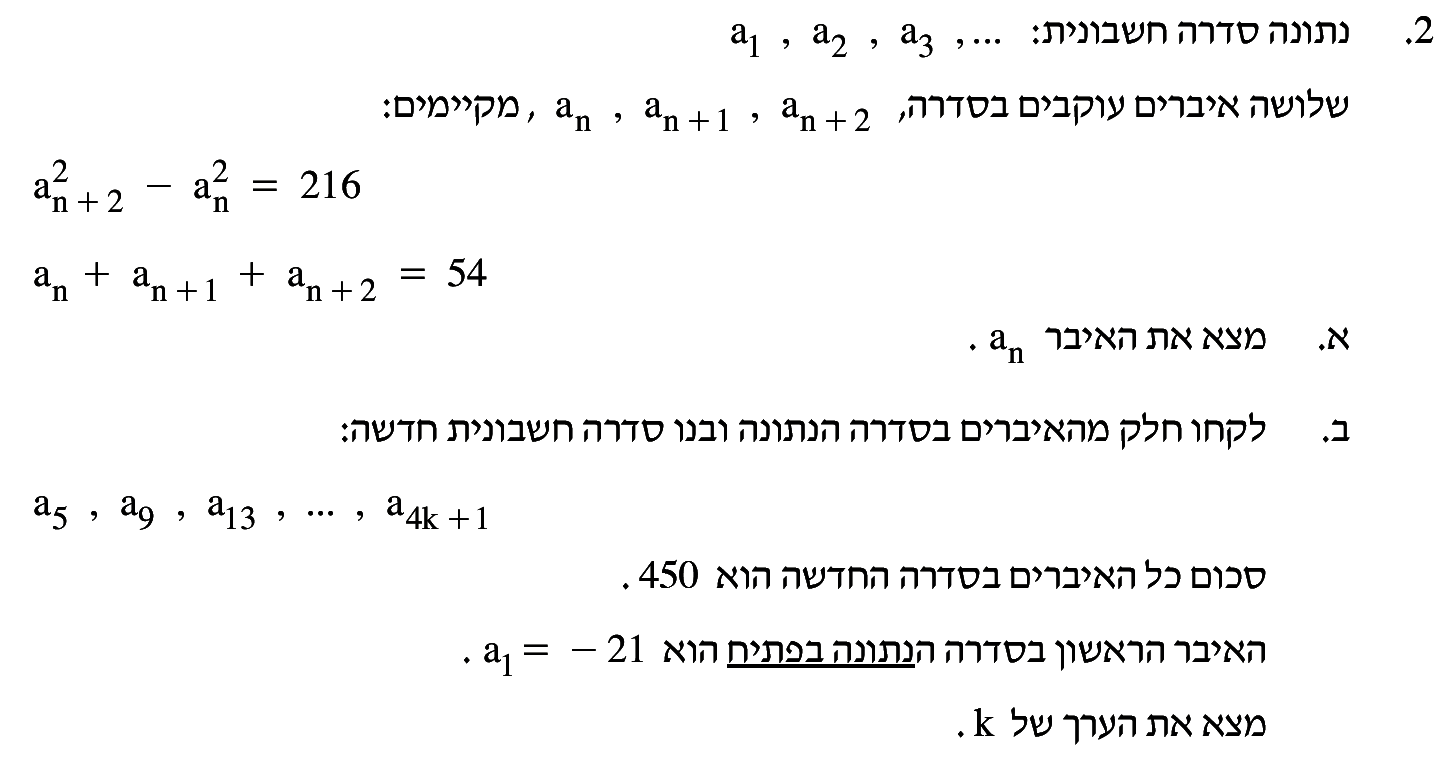
\includegraphics[width=.95\textwidth]{summer-2014b-2}
\end{center}
\vspace{-2ex}


סעיף א. הסדרה חשבונית ולכן ניתן להשתמש בהצבות:
\[
a_{n+1}=a_n+d, \quad a_{n+2}=a_n+2d\,,
\]
כדי לקבל שתי משוואות עם שני נעלמים:
\begin{eqnarray*}
4a_nd+4d^2 &=& 216\\
3a_n + 3d &=& 54\,.
\end{eqnarray*}
ערכי הנעלמים הם
$d=3,a_n=15$.

סעיף ב. הסדרה החדשה חשבונית שאיבריה 
$a'_1, a'_2,\ldots$
הן:
\[
\overbrace{a_5=a_1+4d}^{a_1'}, \quad a_6=a_5+5d,\quad  a_7=a_5+6d,\quad  a_8=a_5+7d,\quad  \overbrace{a_9=a_5+8d}^{a_2'}\,.
\]
בסדרה החדשה:
\[
d' = 8d-4d = 4d = 12\,,\quad\quad\quad a_1' = -21 + 4d= -21 + 12 = -9.
\]
מסכום הסדרה החדשה:
\[
\frac{k}{2}(2a'_1 + (k-1)d')=\frac{k}{2}(-18+(k-1)\cdot 12)=450
\]
נקבלת משוואה ריבועית שהשורש החיובי שלה הוא
$k=10$.


%%%%%%%%%%%%%%%%%%%%%%%%%%%%%%%%%%%%%%%%%%%%%%%%%%%%%%%%%%%%%%%%%%%
\bigskip

\textbf{\R{
חורף תשע"ה
}}

\begin{center}
\selectlanguage{english}
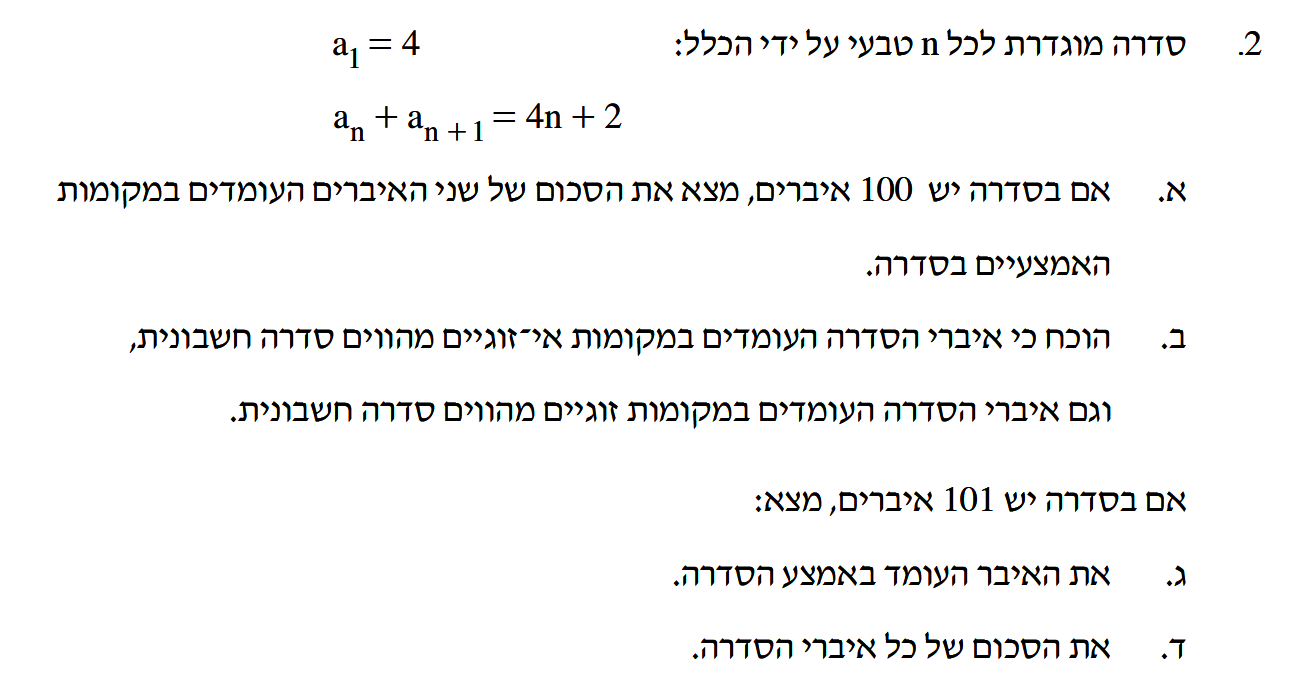
\includegraphics[width=.95\textwidth]{winter-2015-2}
\end{center}
\vspace{-1ex}

סעיף א. כדאי לרשום את הסדרה כדי לוודא מהם האיברים האמצעיים:
\[
\overbrace{\rule{0pt}{8pt}a_1, a_2, \ldots, a_{49}, a_{50}}^{50}, \overbrace{\rule{0pt}{8pt}a_{51}, a_{52},\ldots, a_{100}}^{50}\,.
\]
ניתן לחשב את הסכום מהגדרת הסדרה:
\[
a_{50}+a_{51}=4\cdot 50+2=202\,.
\]
סעיף ב. כדי לחשב את ההפרשים נשתמש ב-"טריק": נוסיף ונחסיר את אותו ערך למשוואה:
\begin{eqnarray*}
a_{k+2} - a_{k} &=& a_{k+2}+(a_{k+1}-a_{k+1})-a_{k}\\
&=& (a_{k+2}+a_{k+1})-(a_{k+1}+a_{k})\\
&=& (4(k+1)+2)-(4k+2)\\
&=&4\,.
\end{eqnarray*}
ההפרש קבוע ולא תלוי בזוגיות, ולכן הזוגיים והאי-זוגיים מהווים סדרות חשבוניות.

סעיף ג. שוב כדאי לרשום את הסדרה:
\[
\overbrace{\rule{0pt}{8pt}a_1, a_2, \ldots, a_{49}, a_{50}}^{50}, a_{51}, \overbrace{\rule{0pt}{8pt}a_{52}, \ldots, a_{100}, a_{101}}^{50}\,.
\]
לא ידוע שהסדרה
$a_{n}$
חשבונית, אבל
$a_{51}$
הוא האיבר ה-%
$25$
בסדרת האי-זוגיים.
$d'=4$
חושב בסעיף ב, ולכן:
\[
a_{51}=a_1+25d' =4+25\cdot 4=104\,.
\]
סעיף ד. נחשב את סכום הסדרה כחיבור של סכום האי-זוגיים וסכום הזוגיים:
$S=S_{\mathit{odd}} + S_{\mathit{even}}$.
$a_1=4$
נתון, וניתן לחשב:
\[
a_2=a_{1+1}=4\cdot 1+2-a_1=4+2-4=2\,.
\]
כבר חישבנו שהפרשים של שתי תת-הסדרות הם 
$4$.
מספר האי-זוגיים הוא
$51$
ומספר הזוגיים הוא
$50$.
הסכום הוא:
\[
S=S_{\mathit{odd}} + S_{\mathit{even}}=\frac{51}{2}(2\cdot 4+50\cdot 4)+\frac{50}{2}(2\cdot 2+49\cdot 4)=5304+5000=10304\,.
\]
\vspace{-4ex}

%%%%%%%%%%%%%%%%%%%%%%%%%%%%%%%%%%%%%%%%%%%%%%%%%%%%%%%%%%%%%%%%%%%
\bigskip

\textbf{\R{
קיץ תשע"ה, מועד א
}}

\begin{center}
\selectlanguage{english}
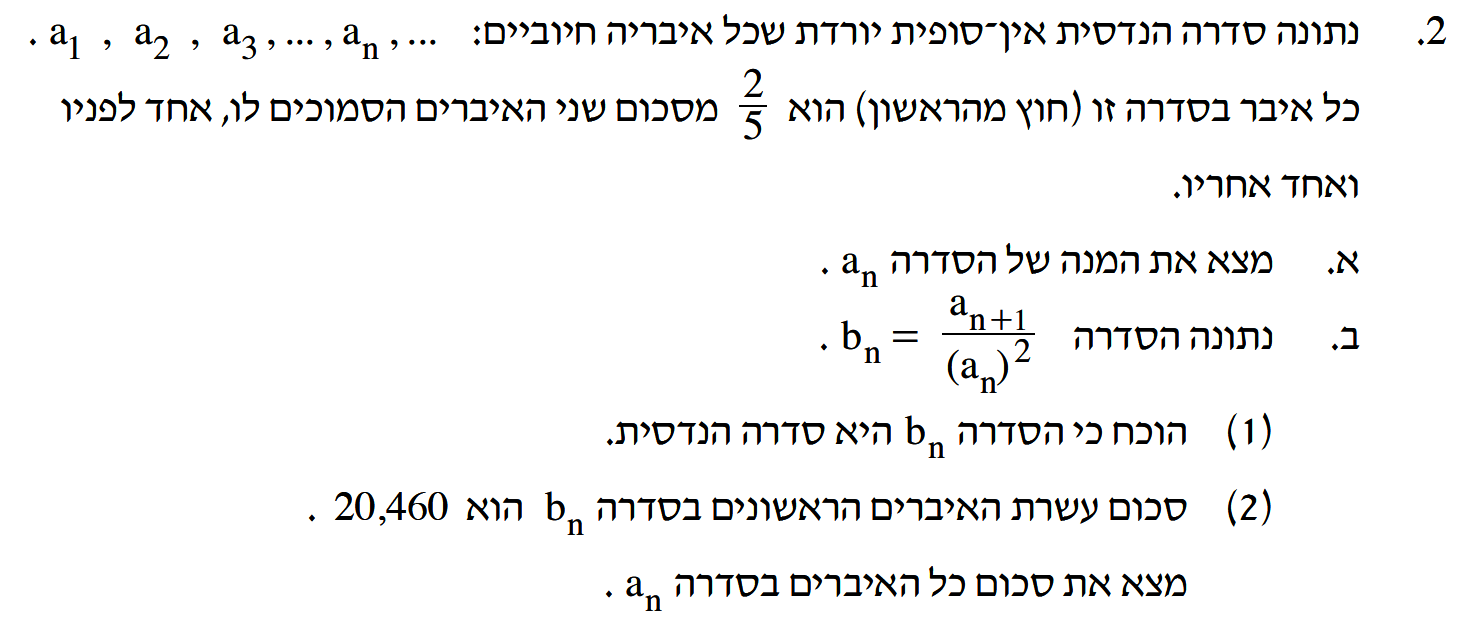
\includegraphics[width=.95\textwidth]{summer-2015a-2}
\end{center}
\vspace{-1ex}
סעיף א. נתון:
\[
a_n = \frac{2}{5}(a_{n-1}+a_{n+1}) =\frac{2}{5}\left(\frac{a_n}{q}+qa_n\right)\,.
\]
$a_n$
מצטמצם ונקבל משוואה ריבועית שפתורונותיה הן 
$q=\frac{1}{2},2$.
נתון שהסדרה יורדת ולכן
$q=\frac{1}{2}$.

סעיף ב
$(1)$.
בחילוק של איברים בסמוכים נציב
$a_{n+1}=a_nq,\;a_{n+2}=a_nq^2$
ונצמצם את
$a_n$:
\[
\frac{b_{n+1}}{b_n} = \frac{\displaystyle\frac{a_{n+2}}{(a_{n+1})^2}}{\displaystyle\frac{(a_{n})^2}{a_{n+1}}}= \frac{a_{n+2}}{(a_{n+1})^2}\cdot\frac{(a_{n})^2}{a_{n+1}} = \frac{q^2}{(q)^2}\cdot\frac{(1)^2}{q}=\frac{1}{q}=2\,.
\]
סעיף ב
$(2)$. 
$b_1=20$
מתקבל מ:
\[
\frac{b_1(2^{10}-1)}{2-1}=20460\,.
\]

השאלה מבקשת את סכום 
\textbf{הסדרה המקורית}
$a_{n}$.
כבר חישבנו את המנה וניתן לחשב את
$a_1$
מהנוסחה עבור 
$b_n$.
החישובים הם:
\[
b_1 = \frac{a_2}{a_1^2} = \frac{qa_1}{(a_1)^2} = \frac{1}{2}\cdot\frac{1}{a_1}\,,\quad\quad\quad a_1=\frac{1}{2b_1}=\frac{1}{40}\,,\quad\quad\quad S_a = \frac{1}{40}\cdot\frac{1}{1-\frac{1}{2}} = \frac{1}{20}\,.
\]
\vspace{-4ex}
%%%%%%%%%%%%%%%%%%%%%%%%%%%%%%%%%%%%%%%%%%%%%%%%%%%%%%%%%%%%%%%%%%%
\bigskip

\textbf{\R{
קיץ תשע"ה, מועד ב
}}

\begin{center}
\selectlanguage{english}
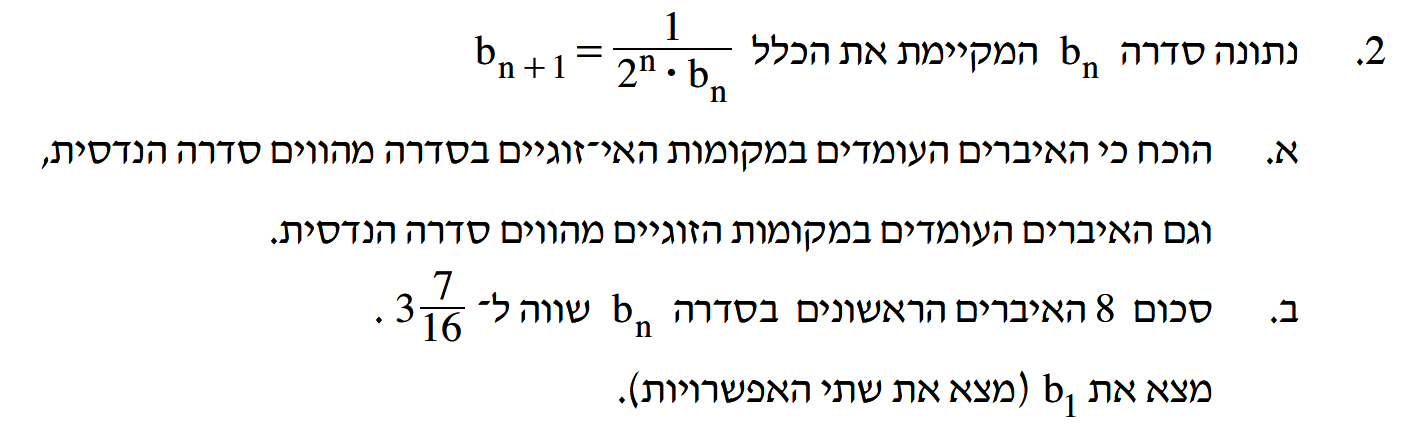
\includegraphics[width=.95\textwidth]{summer-2015b-2}
\end{center}
\vspace{-2ex}
סעיף א. החילוק של איברים במרחק שני מקומות אחד מהשני לא תלוי בזוגיות:
\[
\frac{b_{n+2}}{b_n} = \frac{1}{2^{n+1}b_{n+1}}\cdot\frac{1}{b_n}=\frac{1}{2^{n+1}\cdot\displaystyle\frac{1}{2^nb_n}{b_n}}= \frac{1}{2}\,.
\]
סעיף ב. נחשב בנפרד את הסכום של ארבעת האיברים הזוגיים וארבעת האיברים האי-זוגיים:
\begin{eqnarray*}
S_{\mathit{odd}} &=& b_1+b_3+b_5+b_7=b_1\left(1 + \frac{1}{2} + \frac{1}{4} +\frac{1}{8}\right)=\frac{15}{8}b_1\\
S_{\mathit{even}} &=& b_2+b_4+b_6+b_8=b_2\left(1 + \frac{1}{2} + \frac{1}{4} +\frac{1}{8}\right)=\frac{15}{8}b_2=\frac{15}{8}\cdot\frac{1}{2^1b_1}\,.
\end{eqnarray*}
מ:
\[
S_{\mathit{odd}} + S_{\mathit{even}} =\frac{15}{8}\left(b_1+\frac{1}{2b_1}\right)= 3\frac{7}{16}=\frac{55}{16}\,.
\]
נקבל משוואה ריבועית 
$6b_1^2-11b_1+3=0$
שיש לה שני פתרונות 
$b_1=\frac{3}{2},\,\frac{1}{3}$.


%%%%%%%%%%%%%%%%%%%%%%%%%%%%%%%%%%%%%%%%%%%%%%%%%%%%%%%%%%%%%%%%%%%
\newpage

\textbf{\R{
חורף תשע"ו
}}

\begin{center}
\selectlanguage{english}
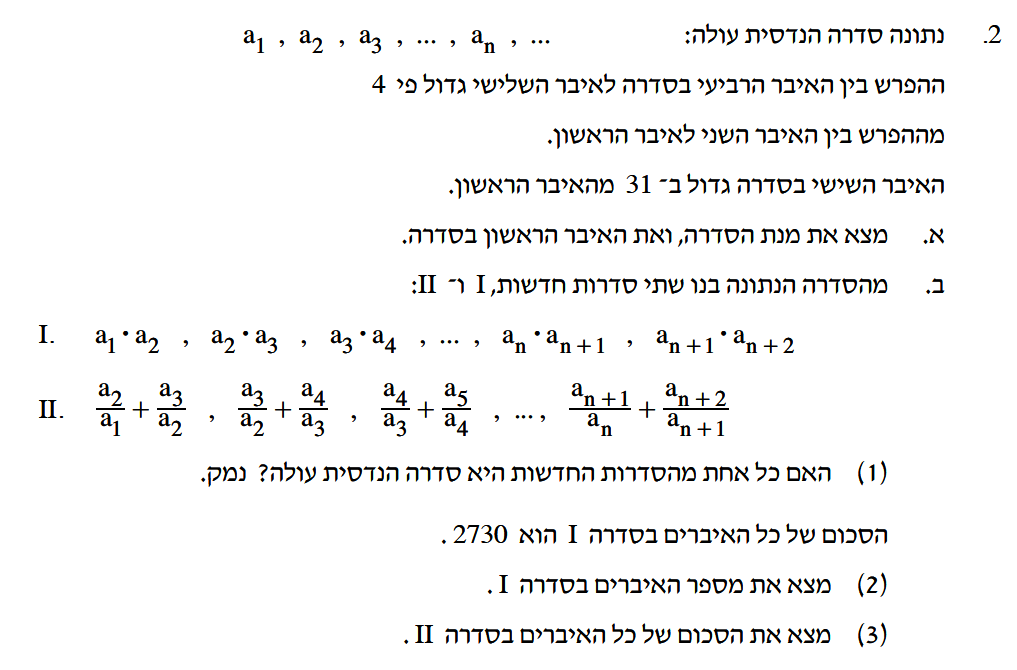
\includegraphics[width=.95\textwidth]{winter-2016-2}
\end{center}

סעיף א. נתון:
\[
(1)\, a_4-a_3 = 4 (a_2-a_1),\quad (2)\, a_6 - a_1 = 31\,.
\]
נציב
$a_n=a_1q^{n-1}$ 
עבור
$a_2, a_3, a_4$,
ב-%
$(1)$,
ונקבל שלוש תשובות
$q=1,q=2,q=-2$.\\
נתון שהסדרה 
\textbf{עולה}
ולכן
$q=2$.
נציב 
$a_1q^5=32 a_1$
עבור
$a_6$
ב-%
$(2)$,
ונקבל
$a_1=1$.

סעיף ב 
$(1)$.
עבור סדרה I:
\[
q_I=\frac{a_{n+1}\cdot a_{n+2}}{a_n\cdot a_{n+1}}=\frac{a_{n+2}}{a_n}=\frac{a_n\,q^2}{a_n}=q^2=4\,,
\]
והסדרה היא סדרה הנדסית עולה. עבור סדרה II:
\[
q_{II}=\left(\frac{a_{n+1}}{a_n} + \frac{a_{n+2}}{a_{n+1}}\right) / \left(\frac{a_{n}}{a_{n-1}} + \frac{a_{n+1}}{a_{n}}\right)=\frac{q+q}{q+q}=1\,.
\]
הסדרה הנדסית אבל
\textbf{לא עולה}.

סעיף
$(2)$.
מסכום הסדרה ניתן לחשב את מספר האיברים בסדרה:
\begin{eqnarray*}
a_1\cdot a_2 + \cdots + a_{n+1} \cdot a_{n+2} &=& 2730\\
(1\cdot 2)\cdot \frac{4^{n+1}-1}{4-1}&=&2730\\
4^{n+1}&=&4096\\
n&=&5\,.
\end{eqnarray*}
\textbf{שימו לב!}
אמנם
$n=5$
אבל מספר האיברים בסדרה I הוא 
$n+1=6$:
\[
(1)\, a_1\cdot a_2,\;\; (2)\,a_2\cdot a_3,\;\;(3)\, a_3\cdot a_4,\;\; (4)\,a_4\cdot a_5,\;\; (5)\,a_5\cdot a_6,\;\; (6)\,a_6\cdot a_7 \;(= a_{n+1}\cdot a_{n+2})\,.
\]
סעיף ב
$(2)$.
חישבנו
$q_{II}=1$.
נחשב את
$a_1^{II}$:
\[
a_1^{II}=\frac{a_{2}}{a_1} + \frac{a_{3}}{a_{2}}=\frac{2}{1}+\frac{4}{2}=4\,.
\]
\textbf{שימו לב!}
מספר האיברים בסדרה II הוא 
$5$:
\[
(1)\,\frac{a_2}{a_1}+\frac{a_3}{a_2},\;\;
(2)\,\frac{a_3}{a_2}+\frac{a_4}{a_3},\;\;
(3)\,\frac{a_4}{a_3}+\frac{a_5}{a_4},\;\;
(4)\,\frac{a_5}{a_4}+\frac{a_6}{a_5},\;\;
(5)\,\frac{a_6}{a_5}+\frac{a_7}{a_6} \left(= \frac{a_{n+1}}{a_n}+\frac{a_{n+2}}{a_{n+1}}\right)\,.
\]
ולכן סכום האיברים הוא:
\[
a_1^{II}+a_1^{II}\cdot 1 + a_1^{II}\cdot 1^2 + \cdots + a_1^{II}\cdot 1^4 = 4\cdot 5=20\,.
\]
\vspace*{-6ex}
%%%%%%%%%%%%%%%%%%%%%%%%%%%%%%%%%%%%%%%%%%%%%%%%%%%%%%%%%%%%%%%%%%%
\bigskip

\textbf{\R{
קיץ תשע"ו, מועד א
}}

\begin{center}
\selectlanguage{english}
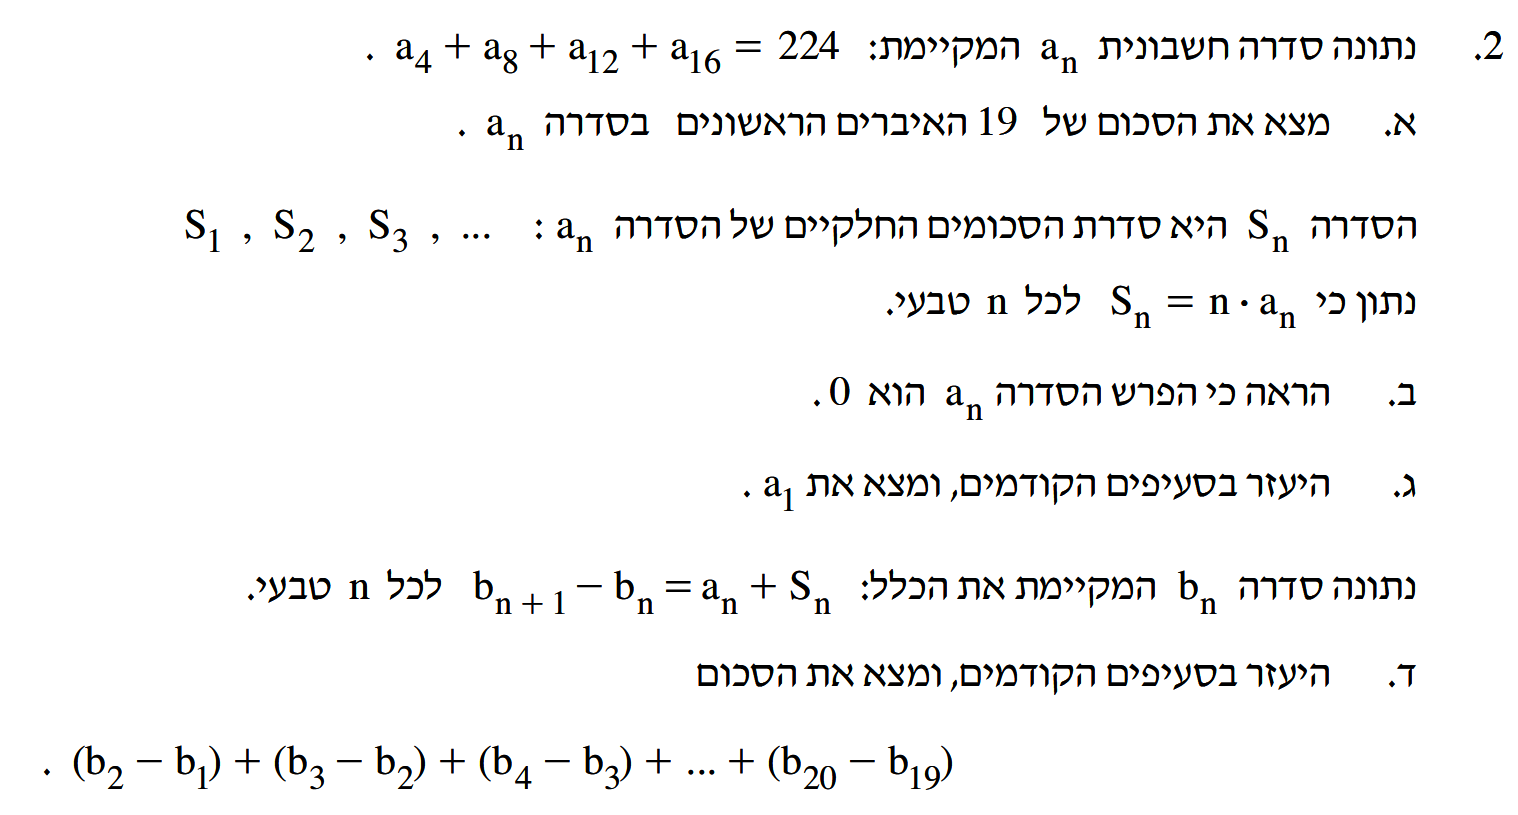
\includegraphics[width=.95\textwidth]{summer-2016a-2}
\end{center}
\vspace{-2ex}
סעיף א. נציב
$a_n=a_1+(n-1)d$
עבור האיברים בסכום ונקבל משוואה אחת עם שני נעלמים:
\begin{eqnarray*}
(a_1+3d)+(a_1+7d)+(a_1+11d)+(a_1+15d)&=&224\\
a_1+9d&=&56\,.
\end{eqnarray*}
לא נתייאש וננסה לחשב את הסכום
$S_{19}$:
\[
S_{19}=\frac{19}{2}(2a_1+18d) = 19(a_1+9d)=19\cdot 56 = 1064\,.
\]
סעיף ב. נשווה את המשוואה הנתונה
$S_n=n\cdot a_n$
לנוסחה עבור סכום של סדרה חשבונית תוך הצבת הנוסחה לאיבר
$a_n$:
\begin{eqnarray*}
n\cdot a_n &=& \frac{n}{2}(2a_1+(n-1)d)\\
n(a_1+(n-1)d) &=&\frac{n}{2}(2a_1+(n-1)d)
\end{eqnarray*}
נפשט את המשוואה ונקבל 
$d=d/2$
שהפתרון היחיד שלה הוא
$d=0$.

סעיף ג. נציב
$0$
עבור 
$d$:
$a_1+9d=a_1+0=56$.

סעיף ד. במבט ראשון נראה שכדאי לצמצם את סכום הסדרה  ל-%
$b_{20}-b_1$,
אבל זה מבוי סתום כי אין לנו דרך לחשב את איברי הסדרה
$b_n$.
במקום זה נחשב את הביטויים
$(b_{i+1}-b_i)$:
\[
b_{i+1}-b_i=a_i+S_i=(a_1+(i-1)\cdot 0)+\frac{i}{2}(2a_1+(i-1)\cdot 0)=a_1(1+i)\,.
\]
הסכום הוא:
\[
a_1(2+3+\cdots+20)=56\cdot\frac{19}{2}(2\cdot 2 + (19-1)\cdot 1)=11704\,.
\]
\vspace{-4ex}


%%%%%%%%%%%%%%%%%%%%%%%%%%%%%%%%%%%%%%%%%%%%%%%%%%%%%%%%%%%%%%%%%%%
\bigskip

\textbf{\R{
קיץ תשע"ו, מועד ב
}}

\begin{center}
\selectlanguage{english}
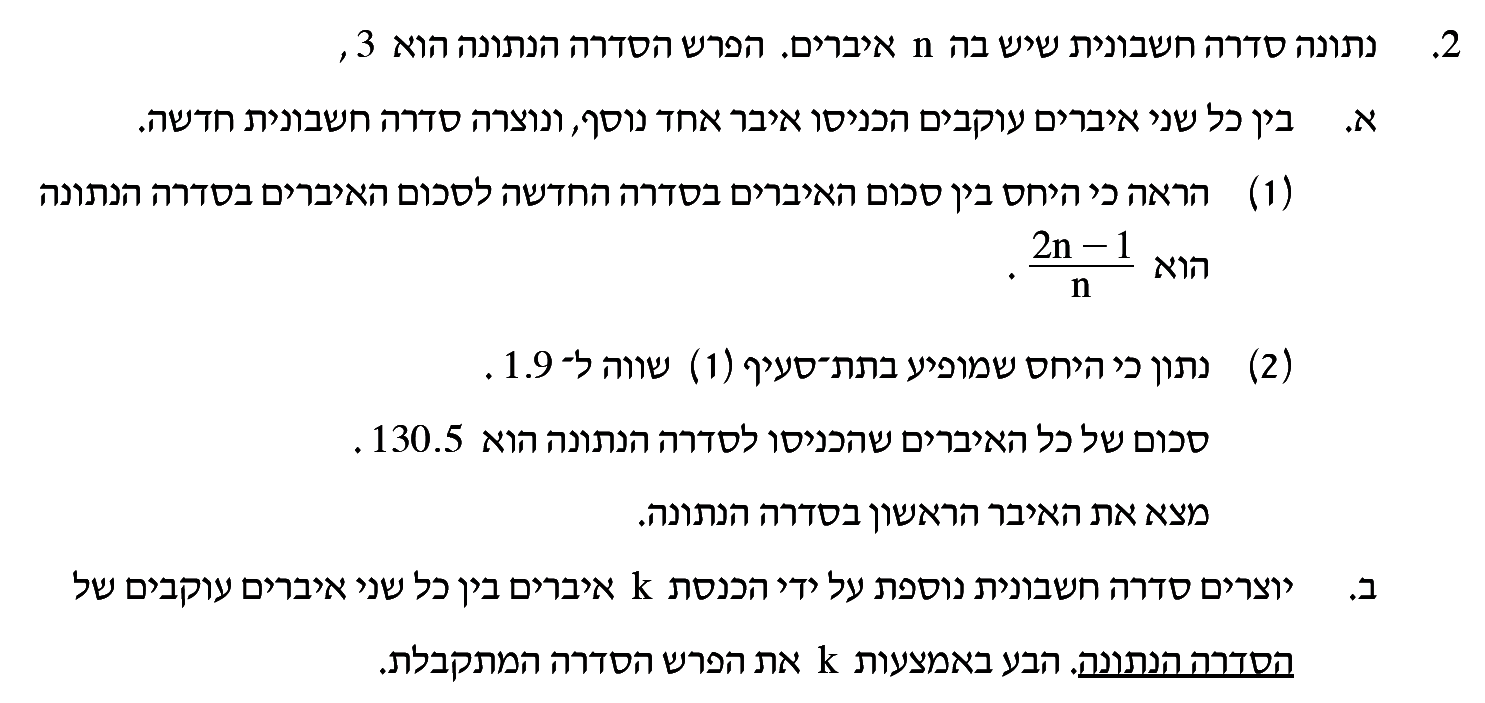
\includegraphics[width=.95\textwidth]{summer-2016b-2}
\end{center}
\vspace{-1ex}
סעיף א
$(1)$.
מספר האיברים החדשים הוא
$n-1$,
כפי שרואים אם רושמים את הסדרה:
\[
a_1,\; a'_1,\; a_2,\; a'_2,\; \ldots,\; a_{n-1},\; a'_{n-1},\; a_n\,.
\]
נתון שהסדרה החדשה גם היא חשבונית. הפרש הסדרה אינו מספר שלם אלא
$1.5$!
המנה של סכומי הסדרות היא:
\[
\frac{S_{\mathit{new}}}{S_{\mathit{old}}}= \frac{\displaystyle\frac{2n-1}{2}(2a_1+1.5(2n-1-1))}{\displaystyle\frac{n}{2}(2a_1+3(n-1))}=\frac{\displaystyle\frac{2n-1}{2}(2a_1+3(n-1))}{\displaystyle\frac{n}{2}(2a_1+3(n-1))}=\frac{2n-1}{n}\,.
\]
סעיף א
$(2)$.
מ-%
$\displaystyle\frac{2n-1}{n}=1.9$
נקבל
$n=10$.

נתון שהסדרה החדשה חשבונית ולכן גם סדרת האיברים החדשים חשבונית:
\[
a'_{i+1}-a'_{i}=a'_{i+1}-(a_{i+1}-a_{i+1})-a'_i=(a'_{i+1}-a_{i+1})+(a_{i+1}-a'_i)=\frac{d}{2}+\frac{d}{2}=3\,.
\]
ניתן לבטא את האיבר הראשון כ-%
$a'_1=a_1+1.5$,
ולחשב את
$a_1$
מהנוסחה לסכום הנתון:
\[
\frac{10-1}{2}(2(a_1+1.5)+((10-1)-1)\cdot 3) = 130.5\,,\quad\quad 9a_1=9\,,\quad\quad a_1=1\,.
\]
סעיף ב. השאלה מכלילה את השאלה בסעיף א על ידי הכנסת
$k$
איברים חדשים בין כל שני איברים סמוכים של הסדרה המקורית. נתון גם שהסדרה החדשה
\textbf{חשבונית},
ולכן ההפרשים בין האיברים החדשים חייבים להיות שווים וסכומם שווה להפרש של הסדרה הנתונה שהוא
$3$.
\[
a_i,\; b_1,\; b_2,\; \ldots,\; b_k,\; a_{i+1}\,.
\]
יש
$k+1$
הפרשים שערכם
$\displaystyle\frac{3}{k+1}$.

%%%%%%%%%%%%%%%%%%%%%%%%%%%%%%%%%%%%%%%%%%%%%%%%%%%%%%%%%%%%%%%%%%%
\bigskip

\textbf{\R{
חורף תשע"ז
}}

\begin{center}
\selectlanguage{english}
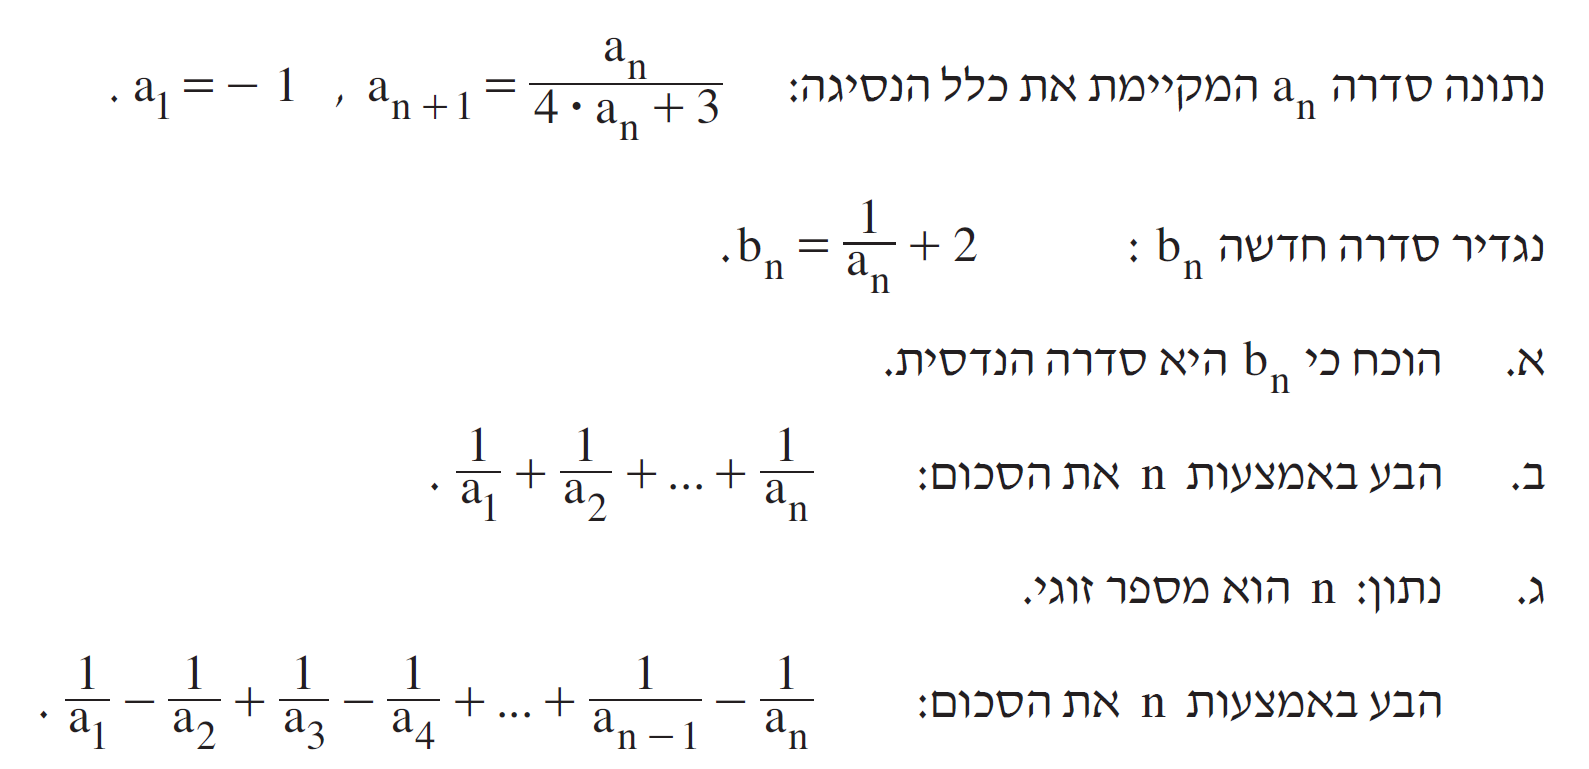
\includegraphics[width=.95\textwidth]{winter-2017-2}
\end{center}
\vspace{-1ex}
סעיף א. נחשב את המנה על ידי הצבה עבור 
$b_n$
לפי ההגדרה, ואחר כך הצבה עבור 
$a_{n+1}$
לפי כלל הנסיגה. נקבל מנה קבועה ולכן הסדרה הנדסית:
\[
\frac{b_{n+1}}{b_n} = \frac{\displaystyle\frac{1}{a_{n+1}}+2}{\displaystyle\frac{1}{a_{n}}+2}= \frac{\displaystyle\frac{4a_n+3}{a_n}+2}{\displaystyle\frac{1}{a_{n}}+2}=\frac{3(2a_n+1)}{2a_n+1}=3\,.
\]
סעיף ב. לא נתון שהסדרה $a_n$ הנדסית, אבל בסעיף א הוכחנו שהסדרה  
$b_n$
הנדסית, ולכן ניתן לבטא את סכום הסדרה
$\displaystyle\frac{1}{a_n}$
כסכום של הסדרה
$b_n$
על ידי ההצבה 
$\displaystyle\frac{1}{a_i} = b_i - 2$:
\[
\frac{1}{a_1} + \cdots + \frac{1}{a_n}=(b_1-2) + \cdots + (b_n-2)=b_1+\cdots+b_n- 2n\,.
\]
בסעיף א חישבנו 
$q_b=3$
ו-%
$b_1=\displaystyle\frac{1}{a_1}+2=\displaystyle\frac{1}{-1}+2=1$.
סכום הסדרה של ההפוכים של 
$a_n$
הוא:
\[
b_1+\cdots+b_n- 2n=\frac{1(3^n-1)}{3-1} - 2n = \frac{3^n - 4n -1}{2}\,.
\]
סעיף ג. לפי ההגדרה של 
$b_n$
נוכל לבטא את הסכום כך:
\[
(b_1 - 2) - (b_2 - 2) + \cdots + (b_{n-1} - 2) + (b_n - 2)\,.
\]
נתון שמספר האיברים זוגי ולכן סכום הקבועים מתאפס. הסכום של איברי
$b_i$
הוא:
\[
b_1-b_2+\cdots+b_{n-1}-b_n=\frac{1((-3)^n-1)}{-3-1}=\frac{3^n-1}{-4}\,.
\]
נתון שמספר האיברים זוגי ולכן סימני השלילה ב-%
$(-3)^n$
מצטמצמים.

%%%%%%%%%%%%%%%%%%%%%%%%%%%%%%%%%%%%%%%%%%%%%%%%%%%%%%%%%%%%%%%%%%%
\bigskip

\textbf{\R{
קיץ תשע"ז, מועד א
}}

\begin{center}
\selectlanguage{english}
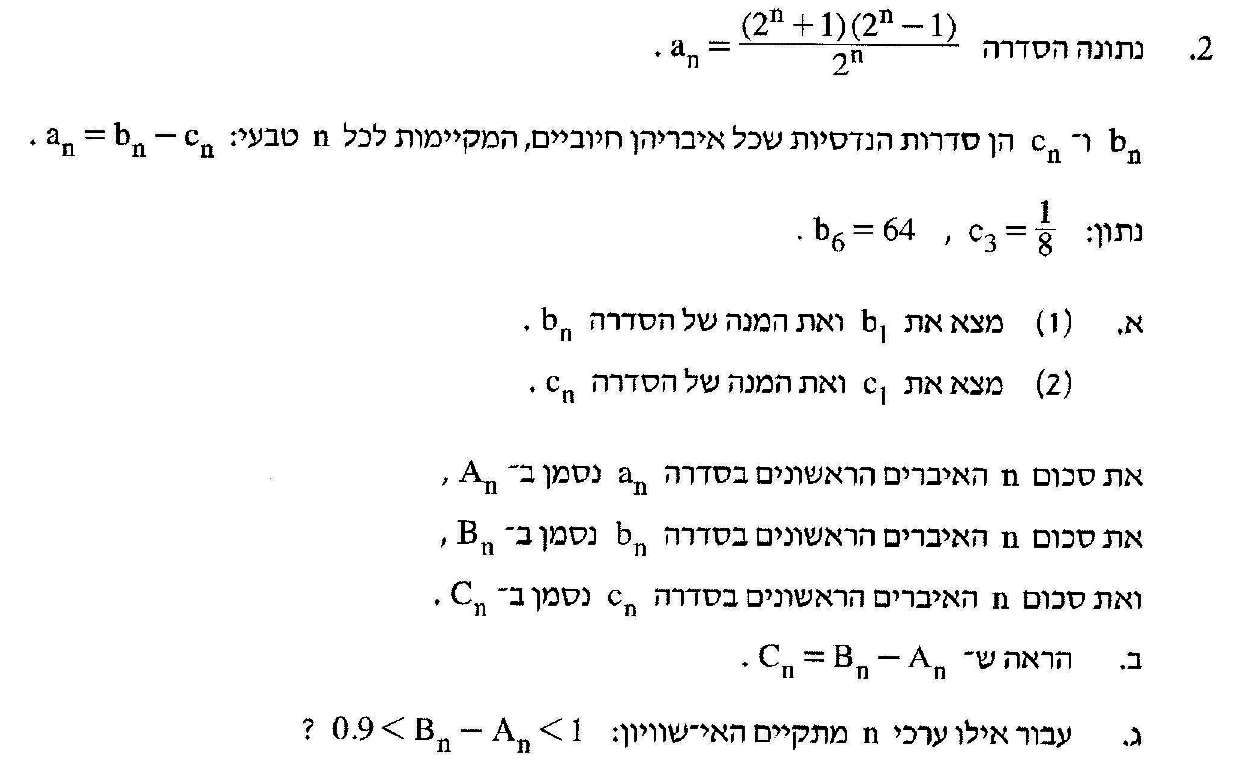
\includegraphics[width=.95\textwidth]{summer-2017a-2}
\end{center}
הנוסחה ל-%
$a_n$
אינה כלל נסיגה כי איברים של הסדרה לא מופיעים בצד הימני של המשוואה. המשוואה מגדריה את
$a_n$
כפונקציה של
$n$.
נתון שהסדרות 
$b_n,c_n$
הנדסיות או לא נתון שום אפיון של הסדרה המקורית
$a_n$.
נחשב ערכים של הסדרה המקורית לפי הפונקציה:
\[
a_3=\frac{(2^3+1)(2^3-1)}{2^3}=\frac{63}{8}\,, \quad\quad a_6=\frac{(2^6+1)(2^6-1)}{2^6}= \frac{65\cdot 63}{64}\,.
\]
סעיף א 
$(1,2)$.
ההגדרה
$a_n=b_n-c_n$
מאפשרת לחשב את הערכים:
\[
b_3=a_3+c_3=\frac{63}{8}+\frac{1}{8}=8\,,\quad\quad c_6=b_6-a_6=64-\frac{65\cdot 63}{64}=\frac{1}{64}\,.
\]
אי אפשר לחשב את מנות של
$b_n,c_n$,
על ידי חילוק של איברים סמוכים כי אין לנו אותם. במקום זה, ננצל את העבודה שנתון שהסדרות הנדסיות כדי לחשב את המנות והאיברים הראשוניים:

\[
\begin{array}{|@{\hspace{2em}}c@{\hspace{2em}}|c|@{\hspace{2em}}c@{\hspace{2em}}|c|}
\hline
\rule[-1.5ex]{0pt}{4ex}b_6&q_b&b_3&b_1\\\hline
\rule[-3.5ex]{0pt}{9ex}b_3q_b^3 & \displaystyle\sqrt[3]{\frac{b_6}{b_3}}=\sqrt[3]{8}=2&
b_1 q_b^2 & \displaystyle\frac{b_3}{q_b^2}=\frac{8}{4}=2\\\hline\hline
\rule[-1.5ex]{0pt}{4ex}c_6&q_c&c_3&c_1\\\hline
c_3q_c^3 & \displaystyle\sqrt[3]{\frac{c_6}{c_3}} =\sqrt[3]{\frac{1}{8}} = \frac{1}{2}&
\rule[-3.5ex]{0pt}{9ex}c_1 q_c^2 & \displaystyle\frac{c_3}{q_c^2}=\frac{1/8}{1/4}=\frac{1}{2}\\
\hline
\end{array}
\]

%\[
%\renewcommand{\arraystretch}{2}
%\begin{array}{l@{\quad\quad\quad}l}
%b_6 = b_3q_b^3 \;\Rightarrow \;q_b = \sqrt[3]{\frac{b_6}{b_3}}=\sqrt[3]{8}=2&
%b_3 = b_1 q_b^2 \;\Rightarrow \;b_1 = \frac{b_3}{q_b^2}=\frac{8}{4}=2\\
%c_6 = c_3q_c^3 \;\Rightarrow \;q_c = \sqrt[3]{\frac{c_6}{c_3}} =\sqrt[3]{\frac{1}{8}} = \frac{1}{2}&
%c_3 = c_1 q_c^2 \;\Rightarrow \;c_1 =\frac{c_3}{q_c^2}=\frac{1/8}{1/4}=\frac{1}{2}\,.
%\end{array}
%\]
סעיף ב. נוכיח תוך שימוש בחוקים של חיבור של מספרים שלמים:
\begin{eqnarray*}
C_n &=& (b_1-a_1) + (b_2 - a_2) + \cdots + (b_n-a_n)\\
&=&(b_1 + b_2 + \cdots + b_n) - (a_1 + a_2 + \cdots + a_n)\\
&=& B_n - A_n\,.
\end{eqnarray*}
סעיף ג. הוכחנו ש-%
$C_n=B_n-A_n$,
ונתונה שהסדרה 
$c_n$
הנדסית. חישבנו 
$q_c=\frac{1}{2},\,c_1=\frac{1}{2}$,
ולכן:
\[
C_n = \frac{1}{2}\cdot\frac{\displaystyle\left(\frac{1}{2}^n-1\right)}{\displaystyle\left(\frac{1}{2}-1\right)}=1-2^{-n}\,.
\]
בדיקה מראה ש-%
$0.9 \not< 1-2^{-3}=0.875$,
אבל
$0.9 < 1-2^{-4}=0.9375 < 1$.

השאלה מבקשת את
\textbf{כל הערכים}
של
$n$
המקיימים את האי-שוויון, ולכן התשובה המליאה היא 
\textbf{כל מספר גדול או שווה ל-}%
$4$,
כי גם עבור מספרים גדולים מ-%
$4$
הביטוי
$1-2^{-n}$
מקיים את האי-שוויון.


%%%%%%%%%%%%%%%%%%%%%%%%%%%%%%%%%%%%%%%%%%%%%%%%%%%%%%%%%%%%%%%%%%%
\bigskip

\textbf{\R{
קיץ תשע"ז, מועד ב
}}

\begin{center}
\selectlanguage{english}
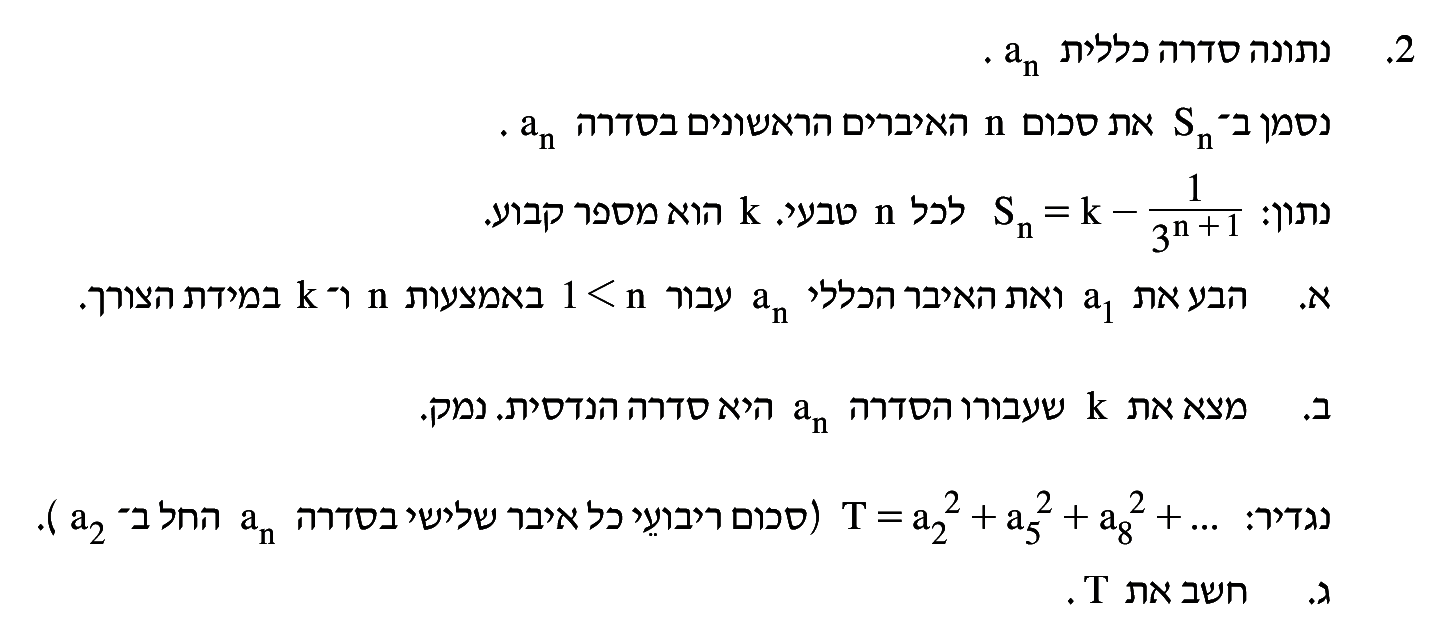
\includegraphics[width=.95\textwidth]{summer-2017b-2}
\end{center}

שאלה זו שונה משאלות אחרות כי נתון ביטוי עבור
\textbf{הסכומים}
ולא עבור האיברים בסדרה.

סעיף א. ניתן לחשב:
\[
a_1=S_1=k-\frac{1}{9}\,, \quad\quad\quad a_n=S_{n}-S_{n-1}=\left(k-\frac{1}{3^{n+1}}\right)-\left(k-\frac{1}{3^{n}}\right)=\frac{2}{3^{n+1}}\,.
\]

סעיף ב. המנה
$q=\displaystyle\frac{a_{n+1}}{a_{n}}=\frac{1}{3}$
לא תלויה ב-%
$k$.
במבט ראשון נראה שהתשובה היא שהסדרה היא הנדסית עבור כל ערך של
$k$,
אולם זו
\textbf{טעות}.
המנה המתקבלת מ-%
$\displaystyle\frac{a_2}{a_1}$
חייבת להיות
\textbf{שווה}
למנה המתקבלת במקרה הכללי
$\displaystyle\frac{a_{n+1}}{a_{n}}$.
נחשב:
\[
\frac{a_2}{a_1}=\frac{\displaystyle\frac{2}{3^3}}{\displaystyle k-\frac{1}{9}} = \frac{a_{n+1}}{a_n}=\frac{1}{3}\,.
\]
הפתרון היחיד הוא
$k=\frac{1}{3}$
ואז האיבר הראשון הוא
$\frac{1}{3}-\frac{1}{9}=\frac{2}{9}$.

סעיף ג. הסדרה החדשה הנדסית כי הסדרה המקורית הנדסית, והמנה של הסדרה החדשה היא המנה המקורית לחזקת
$3\cdot 2=6$:
נבחרו כל איבר שלישי מהסדרה המקורית וכל איבר הוא הריבוע של האיבר המקורי. האיבר הראשון של הסדרה החדשה היא האיבר השני של הסדרה המקורית לחזקת שניים. פתרון אחר הוא לחשב את המנה לפי הנוסחה:
\[
q'=\frac{a_{n+3}}{a_n}=\frac{\left(\frac{2}{3^{n+4}}\right)^2}     {\left(\frac{2}{3^{n+1}}\right)^2}=\left(\frac{1}{3^3}\right)^2=\frac{1}{729}\,.
\]
האיבר הראשון הוא
\[
a'_1 = a_2^2=\left(a_1q\right)^2=\left(\frac{2}{9}\cdot\frac{1}{3}\right)^2=\frac{4}{729}\,,
\]
והסכום הוא:
\[
S'=\frac{a'_1}{1-q'}=
\frac{\displaystyle\frac{4}{729}}{1-\displaystyle\frac{1}{729}}= \frac{1}{182}\,.
\]
%%%%%%%%%%%%%%%%%%%%%%%%%%%%%%%%%%%%%%%%%%%%%%%%%%%%%%%%%%%%%%%%%%%


\textbf{\R{
חורף תשע"ח
}}

\begin{center}
\selectlanguage{english}
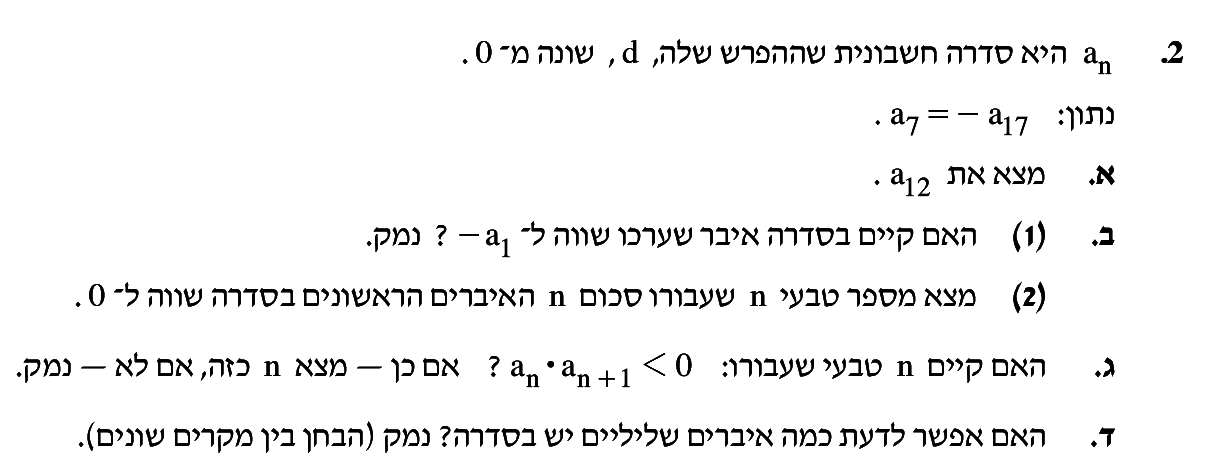
\includegraphics[width=.95\textwidth]{winter-2018-2}
\end{center}


סעיף א. נציב 
$a_1+(n-1)d$
עבור 
$a_7,a_{17}$
ונשתמש במשוואה הנתונה
$a_7=-a_{17}$.
\begin{eqnarray*}
a_1+6d &=& -(a_1+16d)\\
a_1+11d &=& 0\\
a_{12} &=&a_1+11d = 0
\end{eqnarray*}
סעיף ב
$(1)$.
נשווה את
$-a_1$
לנוסחה לאיבר כללי:
\[
-a_1 = a_n = a_1 + (n-1)d\,.
\]
נציב
$a_1=-11d$:
\[
-(-11d) = -11d + (n-1)d\,.
\]
$d$
מצטמצם ונקבל
$n=23$.

סעיף ב
$(2)$.
נציב
$a_1=-11d$
 בנוסחה לסכום של סדרה חשבונית:
\[
\frac{n}{2}(2a_1+(n-1)d) = \frac{n}{2}(2\cdot -11d+(n-1)d) =\frac{dn}{2} (n-23)=0\,.
\]
%\begin{eqnarray*}
%0 &=& \frac{n}{2}(2a_1+(n-1)d)\\
%&=& \frac{n}{2}(2\cdot -11d+(n-1)d)\\
%&=& \frac{dn}{2} (n-23)\,.
%\end{eqnarray*}
נתון שההפרש 
$d$
שונה מאפס וש-%
$n$
מספר טבעי ולכן חיובי, כך שהביטוי מתאפס רק עבור
$n=23$.

סעיף ג. אם איבר חיובי וההפרש חיובי, המכפלה של שני איברים עוקבים היא חיובית, וכך גם אם שניהם שליליים. האפשרות היחידה לקבל מכפלה שלילית היא איבר חיובי והפרש שלילי או להיפך:
\[
\begin{array}{l}
a_k<0,\; a_{k+1}>0\\
a_k>0,\; a_{k+1}<0\,.
\end{array}
\]
אבל ידוע שאחד האיברים בסדרה 
$(a_{12})$
הוא אפס:
\[
\begin{array}{l}
a_k<0,\; a_{k+1}=0,\; a_{k+2}>0\\
a_k>0,\; a_{k+1}=0,\; a_{k+2}<0\,,
\end{array}
\]
ולכן המכפלה של זוג איברים עוקבים חייבת להיות חיובית או אפס.

סעיף ד. נרשום את הסדרה:
\[
a_1,\; a_2,\; \ldots,\; a_{11},\; 0,\; -a_{11},\; \ldots,\; -a_2,\; -a_1,\; \ldots\,.
\]
או ש-%
$11$
האיברים הראשונים שליליים אם ההפרש חיובי, או כל האיברים לאחר האיבר
$a_{12}=0$
שליליים אם ההפרש שלילי.

%%%%%%%%%%%%%%%%%%%%%%%%%%%%%%%%%%%%%%%%%%%%%%%%%%%%%%%%%%%%%%%%%%%
\newpage

\textbf{\R{
קיץ תשע"ח, מועד א
}}

\begin{center}
\selectlanguage{english}
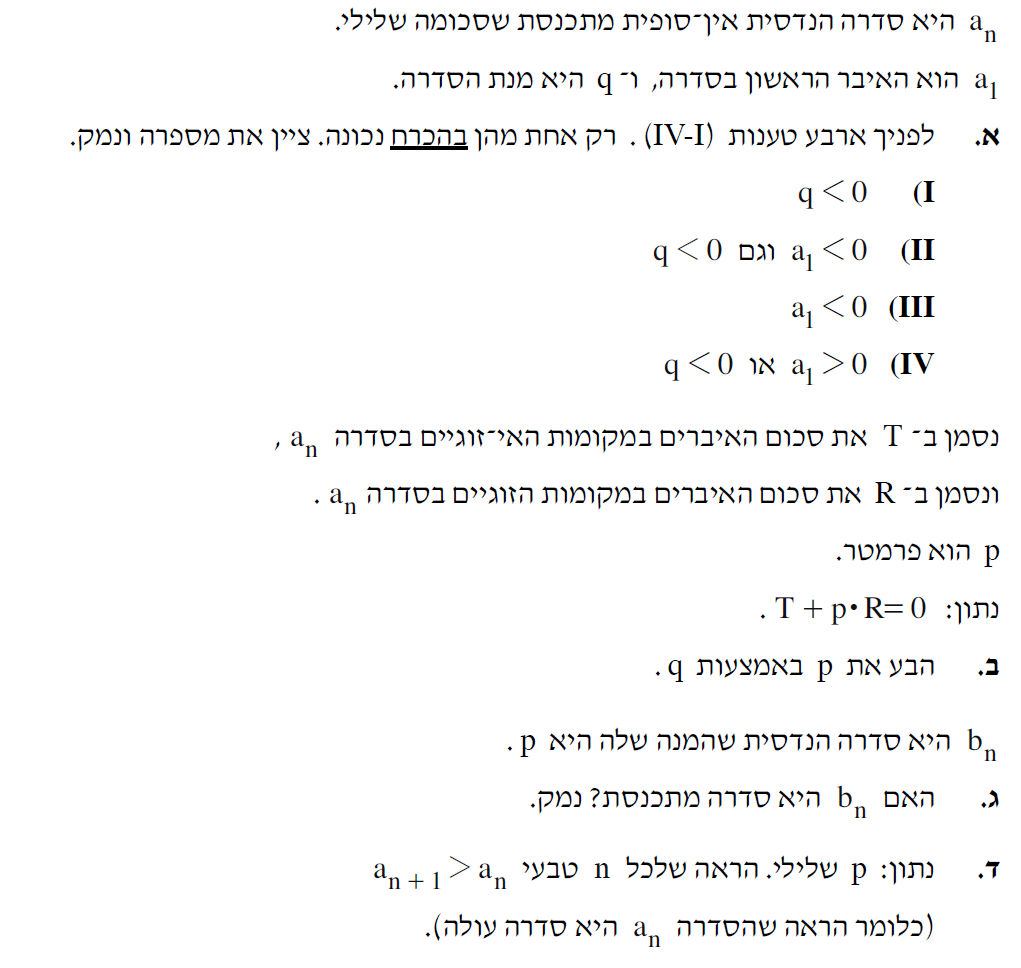
\includegraphics[width=.95\textwidth]{summer-2018a-2}
\end{center}

השאלה בסעיף א יפה כי היא דורשת חשיבה, לא חישובים! נבדוק את הטענות על סדרה מוכרת:
\[
1+ \frac{1}{2} + \frac{1}{4} + \frac{1}{8} + \cdots = 2\,.
\]
אם נהפוך את כל הסימנים למינוס, נקבל סדרה שסכומה שלילי:
\[
-1 - \frac{1}{2} - \frac{1}{4} - \frac{1}{8} - \cdots = -\left(1+ \frac{1}{2} + \frac{1}{4} + \frac{1}{8} + \cdots\right) = -2\,.
\]
ברור שהמנה עדיין חיובית
$\frac{1}{2}$.
לכן אפשר לפסול מייד תשובות 
\L{I, II, IV}
ונשאר רק תשובה
\L{III}.
סדרה הנדסית מתכנסת רק אם
$|q|<1$.
נבדוק: מהנוסחה עבור הסכום:
\[
S = \frac{a_1}{1-q}
\]
ניתן לראות שהסכום שלילי רק אם 
$a_1$
שלילי כי המכנה חיובי
$0 < 1-q < 2$.

סעיף ב. המנה של כל אחת מהסדרות היא
$q^2$
ולכן הסכומים הם:
\[
T = \frac{a_1}{1-q^2},\quad\quad R = \frac{a_1q}{1-q^2}\,.
\]
מהמשוואה הנתונה
$T+pR=0$,
נקבל
$\quad 1+pq=0\quad$
ו-%
$p=-\displaystyle\frac{1}{q}\quad$.

סעיף ג. הסדרה לא מתכנסת כי 
$|q|<1$
גורר
$|p|>1$.

סעיף ד. השאלה שואלת על
\textbf{הסדרה המקורית}
$a_n$
ולא על 
$b_n$.
נתון ש-%
$p$
שלילי ולכן
$q=-\displaystyle\frac{1}{p}$
חיובי. נתון שהסדרה מתכנסת ולכן
$0<q<1$.
מצאנו בסעיף א ש-%
$a_1$
שלילי ולכן
$a_{n+1}>a_n$.
נבדוק בדוגמה: אם 
$a_n=-6,q=\frac{1}{2}$,
אז:
\[
a_{n+1} = a_nq = -6\cdot \frac{1}{2} = -3 \;> \; -6 =a_n\,.
\]

%%%%%%%%%%%%%%%%%%%%%%%%%%%%%%%%%%%%%%%%%%%%%%%%%%%%%%%%%%%%%%%%%%%

\textbf{\R{
קיץ תשע"ח, מועד ב
}}

\begin{center}
\selectlanguage{english}
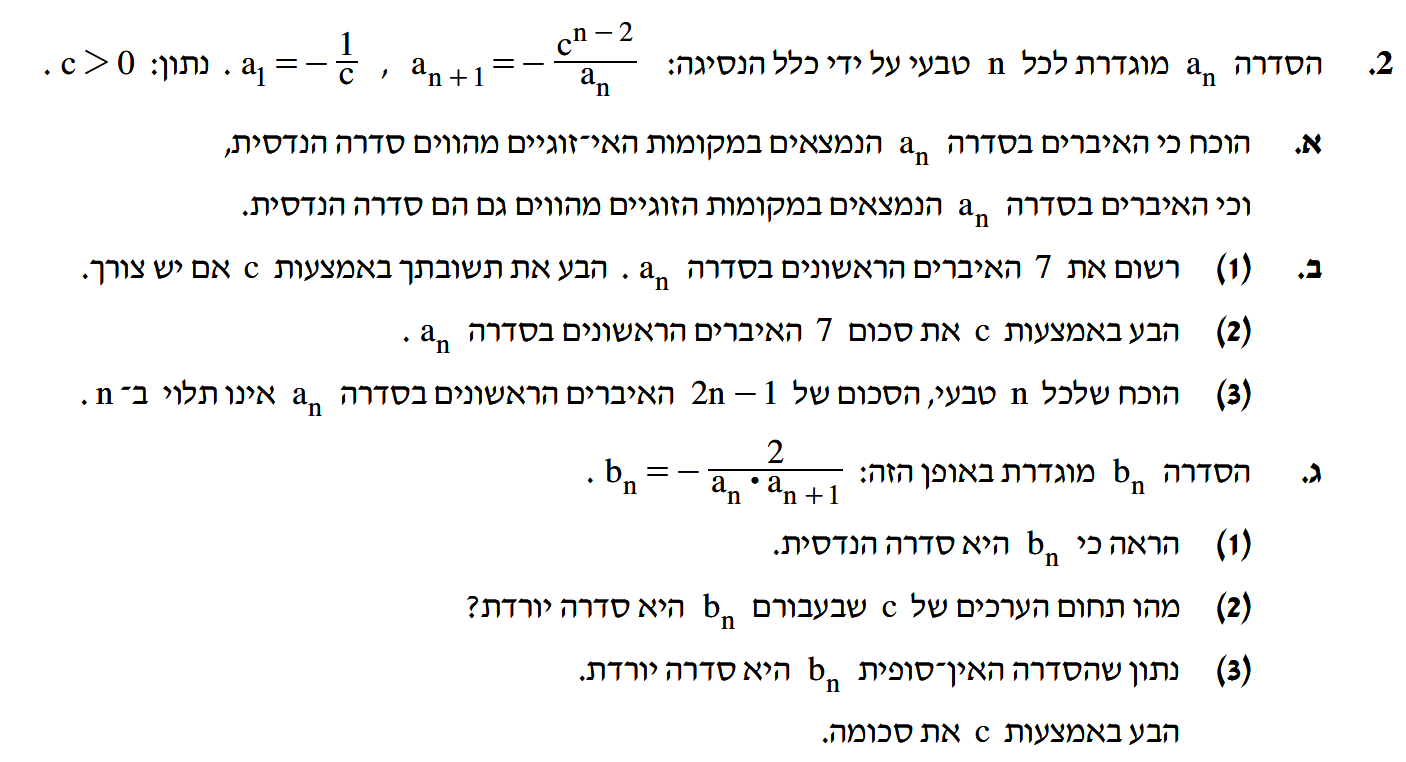
\includegraphics[width=\textwidth]{summer-2018b-2}
\end{center}
\vspace{-2ex}
סעיף א. נציב את כלל הנסיגה בתוך עצמו:
\[
a_{n+1} = -\frac{c^{n-2}}{a_n} = -\frac{c^{n-2}}{\displaystyle -\frac{c^{n-3}}{a_{n-1}}} = ca_{n-1}\,.
\]
המנה
$a_{n+1}/a_{n-1}=c$
קבועה לא תלוי בזוגיות של האיברים.

סעיף ב
$(1)$.
הסדרות של הזוגיים והאי-זוגיים הן סדרות הנדסיות
\textbf{נפרדות},
ולכן יש לחשב את האיברים
$(a_1,a_3,a_5,a_7), (a_2,a_4,a_6)$
בנפרד:
\[
\renewcommand{\arraystretch}{2}
\begin{array}{l}
a_1=-\displaystyle\frac{1}{c},\;\;a_3=ca_1=-1,\;\;a_5=ca_3=-c,\;\;a_7=ca_5=-c^2\\
a_2=\displaystyle
-\frac{c^{1-2}}{a_1}=
-\frac{c^{-1}}{-\frac{1}{c}}=1,\;\;a_4=ca_2=c,\;\;a_6=ca_4=c^2\,.
\end{array}
\]
סעיף ב
$(2)$.
כאשר מסכמים את האיברים הם מצטמצמים פרט לאיבר הראשון, ולכן
$S_7=-\frac{1}{c}$.

סעיף ב
$(3)$.
יש 
$n$ 
אי-זוגיים ו-%
$n-1$
זוגיים, ראו את הפתרון לבחינה של
\textbf{קיץ תשע"ו ב}:
\[
S_{\mathit{odd}}+S_{\mathit{even}}=-\frac{1}{c}\frac{c^n-1}{c-1}+ 1\cdot\frac{c^{n-1}-1}{c-1}= \frac{-c^{n-1}+c^{-1} + c^{n-1}-1}{c-1}= -\frac{1}{c}\,.
\]
סעיף ג
$(1)$.
\[
\frac{b_{n+1}}{b_n} = \frac{\displaystyle\frac{2}{a_{n+1}a_{n+2}}}{\displaystyle\frac{2}{a_{n}a_{n+1}}}= \frac{a_n}{a_{n+2}} =  \frac{1}{\displaystyle\frac{a_{n+2}}{a_n}} = \frac{1}{c}\,.
\]
סעיף ג
$(2)$.
סדרה יורדת אם
$0<q=\displaystyle\frac{1}{c} < 1$.
נתון
$c>0$,
ולכן הסדרה יורדת אם
$c>1$.

סעיף ג
$(3)$.
נתון שהסדרה היא הנדסית אינסופית יורדת. ניתן להשתמש בנוסחה 
$S=\displaystyle\frac{a_1q}{1-q}$:
\[
b_1=\frac{-2}{a_1a_2}= \frac{-2}{\displaystyle-\frac{1}{c}\cdot 1}=2c\,,\quad\quad
S_b = 2c\cdot\frac{1}{1-\displaystyle\frac{1}{c}}=\frac{2c^2}{c-1}\,.
\]



%%%%%%%%%%%%%%%%%%%%%%%%%%%%%%%%%%%%%%%%%%%%%%%%%%%%%%%%%%%%%%%%%%%

\newpage

\begin{center}
\textbf{המלצות}
\end{center}

\begin{itemize}


\item
\textbf{חובה לקרוא את השאלות בזהירות רבה.}
בבחינה של
\textbf{קיץ תשע"ה א},
סעיף ב שואלת על סדרה חדשה
${b_n}$
אבל בסוף חוזרת ומבקשת למצוא את הסכום של הסדרה הנתונה
${a_n}$.

\item
שימו לב אם סדרה היא חשבונית, הנדסית או לא זו ולא זו. אני מציע להדגיש את המילים "חשבונית" ו-"הנדסית" בשאלה.

\item 
ברוב השאלות נתונה סדרה ומוגדרת סדרה חדשה המובססת על הסדרה הנתונה. 
\textbf{אין בהכרח קשר}
בין תכונה של הסדרה המקורית והסדרה החדשה. להלן שתי סדרות חשבוניות, אבל כאשר משלבים את שתיהן, מתקבלת סדרה שאיננה חשבונית:
\[
\begin{array}{rrrrrrrrrrr}
1,& 4,& 7,& 10,& 13,& \ldots\\
2,& 5,& 8,& 11,& 14, &\ldots\\
1,& 2,& 4,& 5,& 7,& 8,& 10,& 11,& 13,& 14, &\ldots
\end{array}
\]
בבחינה של
\textbf{חורף תשע"ד}
נתונה סדרה הנדסית אבל השאלה מבקשת להוכיח שסדרת ההפוכים של האיברים הגם היא הנדסית.

\item
כאשר מבקשים להוכיח שתת-סדרת הזוגיים חשבונית או הנדסית וגם תת-סדרת האי-זוגיים )בחינה של
\textbf{קיץ תשע"ה ב}%
(, הוכחה אחת תספיק כי אם 
$\displaystyle \frac{a_{n+2}}{a_n}$
קבועה, לא משנה אם 
$n$
זוגי או אי-זוגי.


\item

כדאי לרשום את איברי הסדרה במיוחד כאשר שואלים על איברים זוגיים ואי-זוגיים )בחינה של
\textbf{חורף תשע"ה}(:
\[
\begin{array}{l}
\overbrace{\rule{0pt}{8pt}a_1, a_2, \ldots, a_{49}, a_{50}}^{50}, \overbrace{\rule{0pt}{8pt}a_{51}, a_{52},\ldots, a_{100}}^{50}\\
\underbrace{\rule{0pt}{8pt}a_1, a_2, \ldots, a_{49}, a_{50}}_{50}, a_{51}, \underbrace{\rule{0pt}{8pt}a_{52}, \ldots, a_{100}, a_{101}}_{50}\,.
\end{array}
\]
\vspace{-4ex}

\item
מקרה מעניין הוא תת-סדרות חופפות )בחינה של 
\textbf{חורף תשע"ב}
שלא נמצאת במסמך זה(:
\[
\renewcommand{\arraystretch}{.4}
\begin{array}{ll}
\overbrace{\rule{0pt}{8pt}a_1, a_2, \ldots, a_n}^{n},&\hspace{-9pt}a_{n+1}, a_{n+2}, \ldots, a_{2n-1}\\
&\hspace{-2em}\underbrace{\rule{10em}{0pt}}_{n}
\end{array}
\]
\vspace{-4ex}
\item
קיימות שתי דרכים לסכם מספר תת-סדרות )בחינה של
\textbf{קיץ תשע"ד א}%
(. דרך אחת היא לסכם כל תת-סדרות בנפרד עם ערכי ה-%
$d, a_1$
או
$n, q$
שלהן. זה קורה לעתים קרובות כאשר השאלה מבקשת לחשב סכום של סדרה, אבל ידוע רק שתת-סדרות חשבוניות או הנדסיות, למשל, זוגיים ואי-זוגיים )בחינה של
\textbf{קיץ תשע"ח ב}(.
\item 
דרך אחרת היא לחבר הסכומים של תת-סדרות ולהחסיר את התוצאה מסכום הסדרה כולה:
\[
S_1 = S_n - (S_2+S_3)\,.
\]
\vspace{-6ex}

\item
בסדרה קיימים ארבעה נעלמים
$d, a_1$
או
$S, n, q$.
כדי למצוא את ערכו של נעלם אחד, צריך לדעת את ערכי שלושת הנעלמים האחרים )או שניים אם לא מדובר בסכום(. אם מבקשים לבטא נעלם אחד באמצעות בנעלם אחר, אפשר להסתדר עם פחות ערכים. לפעמים, מספיק לדעת את הקשר בין שני נעלמים כדי לפתור בעיה, כגון
$a_1+11d = 0$
בבחינה של
\textbf{הורף תשע"ח}.

\item
הבחינה של
\textbf{חורף תשע"ו}
מעניינת כי מספר האיברים הוא לא הערך של מספר 
$n$
המופיע בשאלה. חשוב לרשום דוגמה מספרית כדי לוודא מהו מספר האיברים:
\[
(1)\, a_1\cdot a_2,\;\; (2)\,a_2\cdot a_3,\;\;\cdots\;\; (5)\,a_5\cdot a_6=(a_n\cdot a_{n+1}),\;\; (6)\,a_6\cdot a_7 \;(= a_{n+1}\cdot a_{n+2})\,.
\]

\item
טריק שימושי הוא לחבר ולהחסיר את אותו ערך בביוטי )בחינה 
\textbf{חורף תשע"ה}(:
\[
a_{k+2} - a_{k} = a_{k+2}+(a_{k+1}-a_{k+1})-a_{k} = (a_{k+2}+a_{k+1})-(a_{k+1}+a_{k})\,.
\]

\item
הכנסת איברים חדשים בתוך סדרה לא בהכרח שומרת על הסדרה כחשבונית או הנדסית. השורה הראשונה להלן היא סדרה חשבונית. בשורה השנייה הוכנסו איברים של סדרה חשבונית נוספת והסדרה החדשה היא חשבונית. בשורה השלישית הוכנסו איברים של סדרה חשבונית נוספת והסדרה החדשה איננה חשבונית.
\[
\begin{array}{rrrrrrrrrrrrr}
1,& 5,& 9,& 13,& 17\\
1, &3,& 5,&7,& 9,& 11,& 13, &15, & 17\\
1, &2,& 5,&6,& 9,& 10,& 13, &14, & 17
\end{array}
\]
בבחינה של
\textbf{קיץ תשע"ו ב}
כתוב במפורש שהסדרה חדשה חשבונית.

\item
בישוב הפרש או מנה, כדאי להציב ב-%
$a+{n+1}$
ביוטי שיש בו 
$a_n$.
הנה דוגמה מהבחינה של 
\textbf{קיץ תשע"ה א}:
\[
a_n = \frac{2}{5}(a_{n-1}+a_{n+1}) =\frac{2}{5}\left(\frac{a_n}{q}+qa_n\right)\,.
\]
$a_n$
מצטמצם ונקבל משוואה ריבועית ב-%
$q$.

\end{itemize}

\end{document}
